\documentclass[aps, prc, 12pt, nofootinbib, showpacs, superscriptaddress, tightenlines, groupedaddress]{revtex4-2}
\usepackage{amsmath,amssymb,amsbsy,bm}
\usepackage{graphicx}
\usepackage{comment}
\usepackage{float}
\usepackage[colorlinks=true,linkcolor=blue,citecolor=blue,urlcolor=blue]{hyperref}
\usepackage[margin=0.75in]{geometry}
\usepackage{silence}
\WarningFilter{revtex4-2}{Repair the float}

%\usepackage[table]{xcolor}

\begin{document}

\title{Baryon Transport in Color Flux Tubes}
\author{Scott Pratt}
\affiliation{Department of Physics and Astronomy and National Superconducting Cyclotron Laboratory\\
Michigan State University, East Lansing, MI 48824~~USA}
\date{\today}

\pacs{}

\begin{abstract}
baryon transport ...
\end{abstract}

\maketitle

\section{Introduction}

\section{Baryon Transport from Merging Simple Flux Tubes}

Here, we consider the merging of two simple flux tubes into one. The term ``simple'' refers to the fact that the tube is generated by a single quark or anti-quark. In a simple tube, one can bisect the tube at any point and classify the color charge on each side of the bisection by its color multiplet, $p,q$. In SU(3), the multiplet is defined by two integers, which differs from SU(2), where a multiplet is denoted by a single number, $j$, e.g. the total angular momentum. Graphically, the state can be enumerated by the graphs in Fig. \ref{fig:pqmultiplet}. Multiplets denoted by $(p_1,q_1)$ and $(p_2,q_2)$ can be combined to create multiplets denoted by $(p',q')$. In SU(2), multiplets denoted by $j_1$ and $j_2$ only couple to singlet $j'=0$ if $j_1=j_2$. Similarly, for SU(3) two multiplets couple to a color singlet only if $p_1=q_2$ and $p_2=q_1$. For example, the $(1,0)$ multiplet (quark) and the $(0,1)$ multiplet (antiquark) can couple to a color singlet.

Before addressing merging, we review the case of a simple flux tube between a quark and antiquark. Figure \ref{fig:simpletube} illustrates how the flux can be reduced by quark-antiquark pairs tunneling out of the vacuum. 
\begin{figure}
\centerline{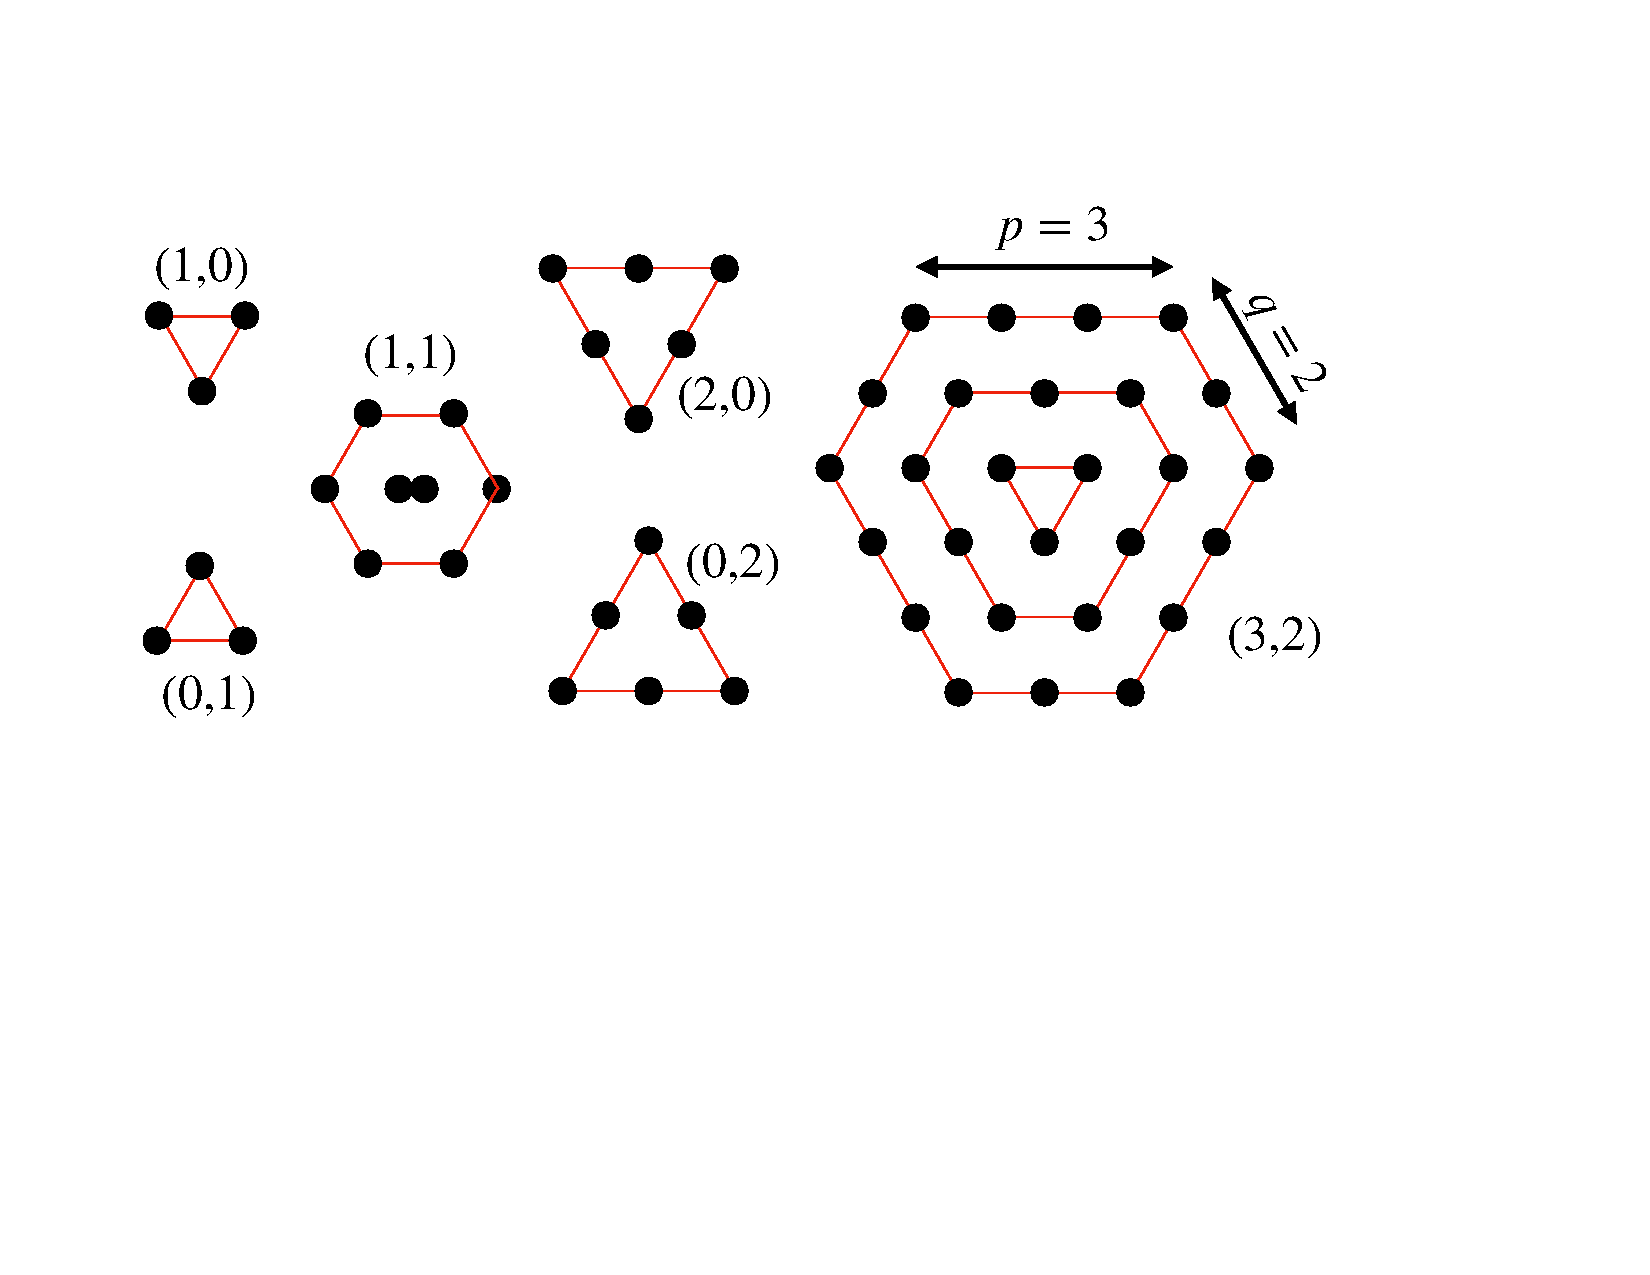
\includegraphics[width=0.6\textwidth]{figs/pqmultiplet.pdf}}
\caption{\label{fig:pqmultiplet}
Graphical representation of $(p,q)$ multiplets. The quark and antiquark color{} triplets are represented by $(1,0)$ and $(0,1)$, respectively, while the gluon octet is $(1,1)$. Each dot represents one projection of the multiplet, if the dot is on the outer ring. Subsequently, for the next inner-ring ring a dot represents two states, or three states for the next inner-ring, although the increasing degeneracy stops once a ring has either $p=0$ or $q=0$. The net degeneracy of the multiplet is $(p+1)(q+1)(p+q+2)/2$. In SU(2) one can combine multiplets of $j_1$ and $j_2$ to form several multiplets $j'$. Similarly, in SU(3) one can combine multiplets of $(p_1,q_1)$ and $(p_2,q_w)$ to form multiplets of several combinations of $(p',q')$.
}
\end{figure}

....

\begin{figure}
\centerline{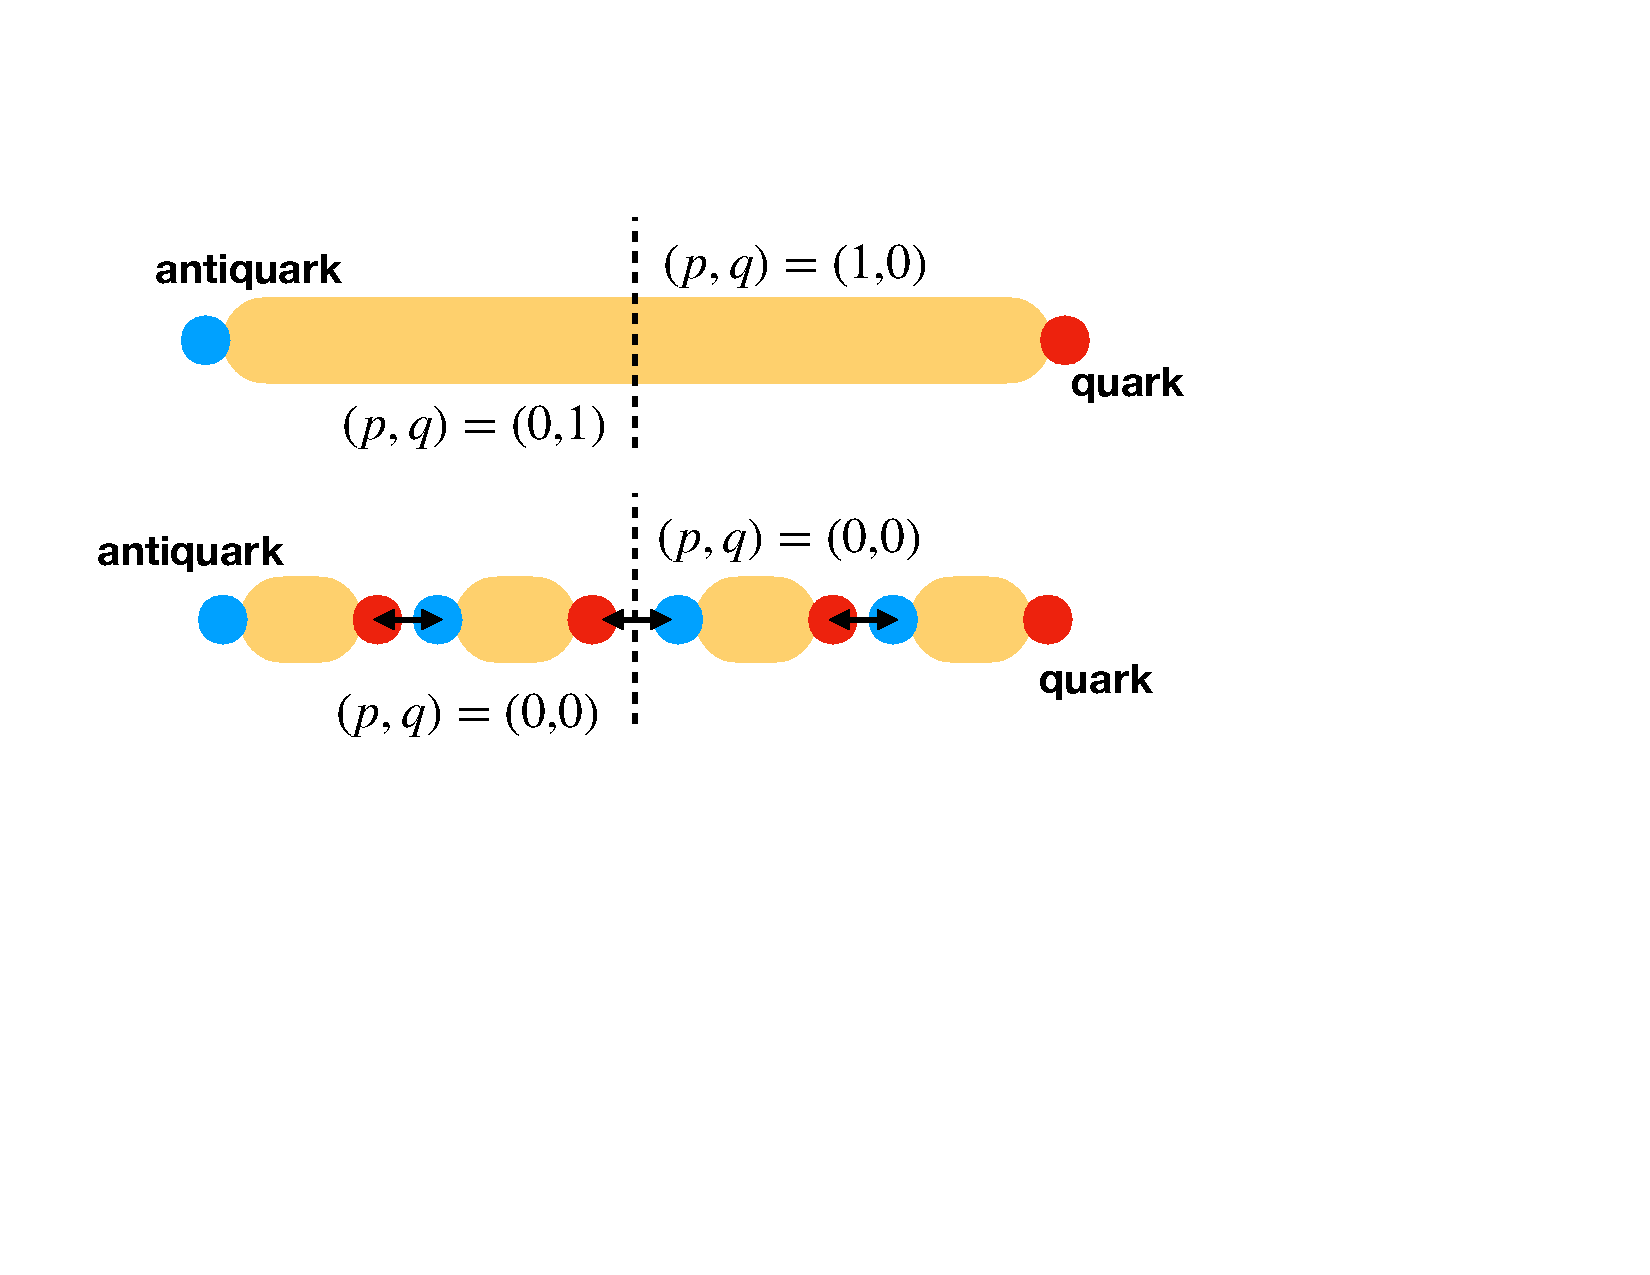
\includegraphics[width=0.4\textwidth]{figs/simpletube.pdf}}
\caption{\label{fig:simpletube}
A simple flux tube between a quark $(p=1,q=0)$ and an antiquark $(p=0,q=1)$ is illustrated in the upper panel, with the lighter and darker circles representing the quark and antiquark respectively. Drawing a vertical line through a flux tube divides space into two regions, the left side of the dashed line in a color multiplet $(p=1,q=0)$ and the right side in the multiplet $(p=0,q=1)$. The lower panel illustrates how quark-antiquark pairs can tunnel out of the vacuum so that the space between the tunneling quarks is free of color fields. Tunneling quark-antiquark pairs are denoted by the arrows.  Dividing space that does not bisect a tube results in both sides being in color singlets.
}
\end{figure}


\begin{figure}
\centerline{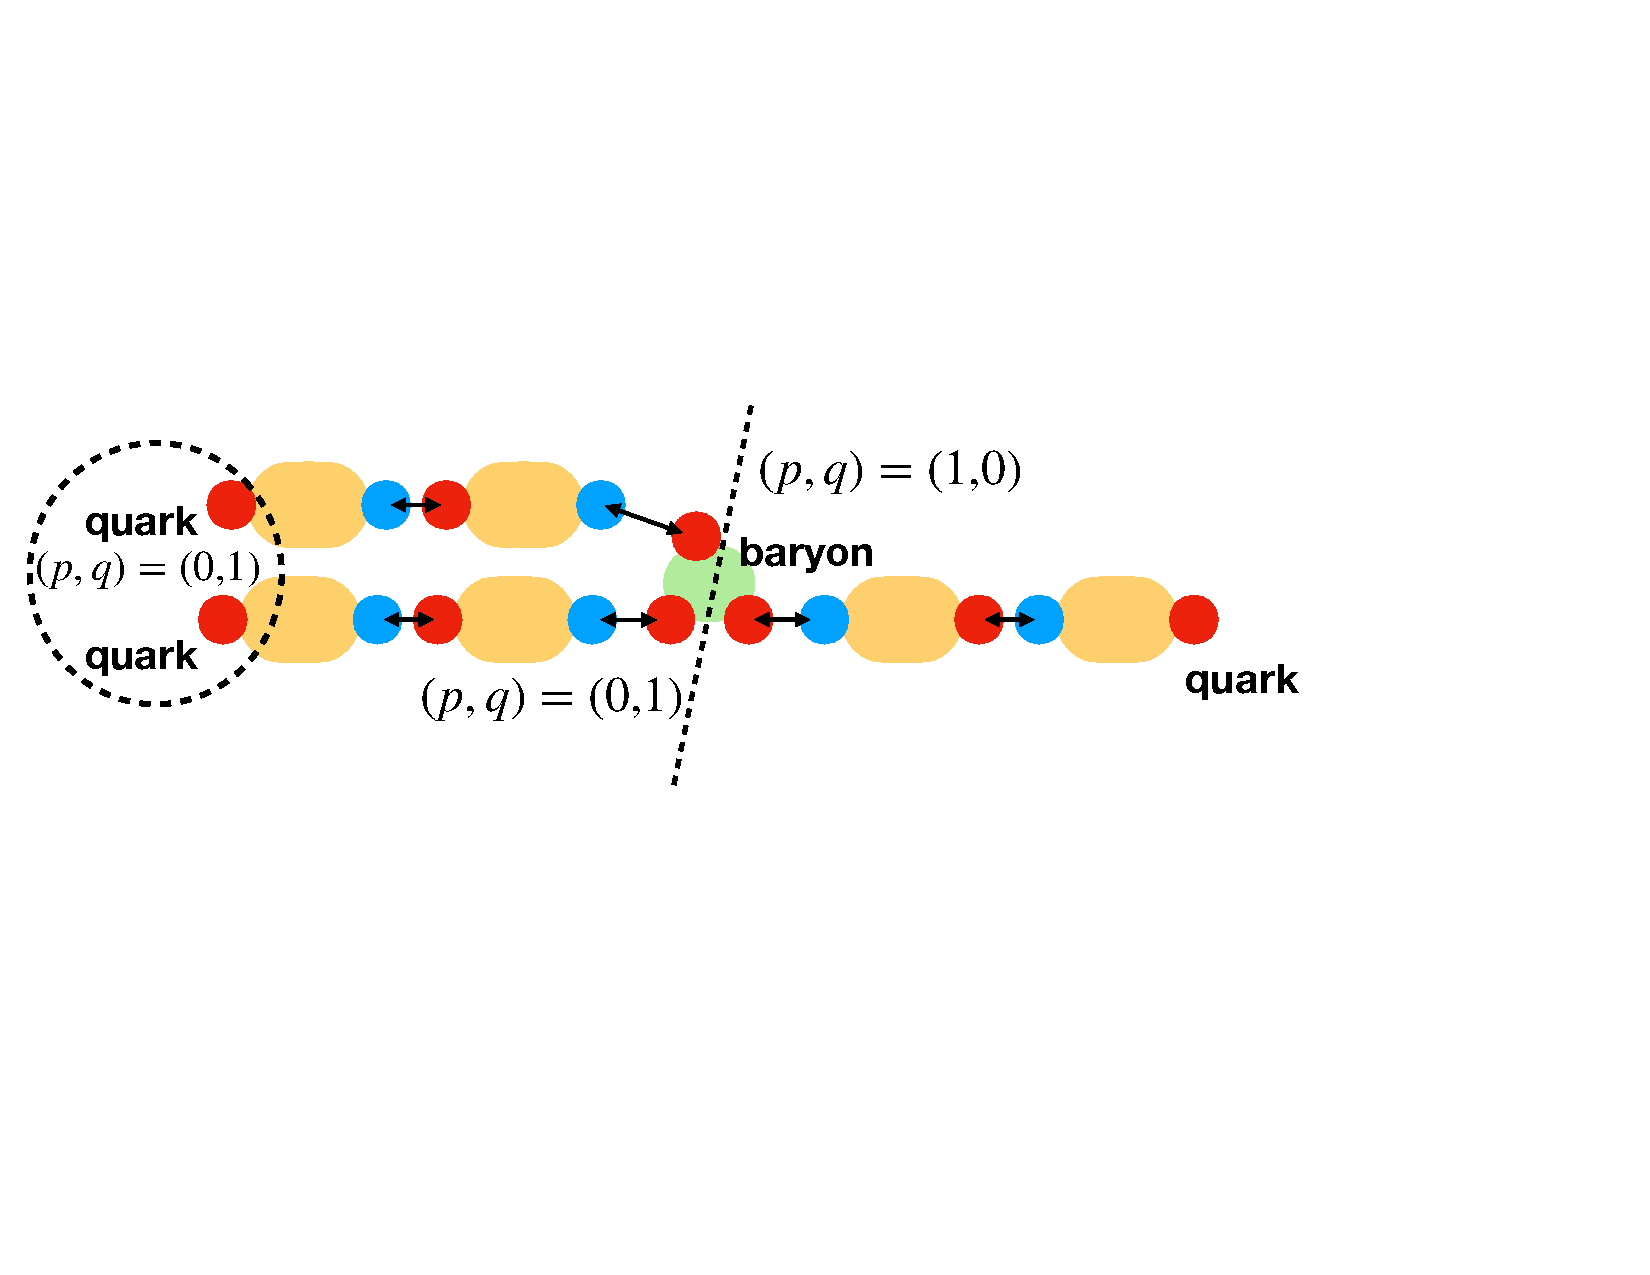
\includegraphics[width=0.48\textwidth]{figs/simplemerge.pdf}}
\centerline{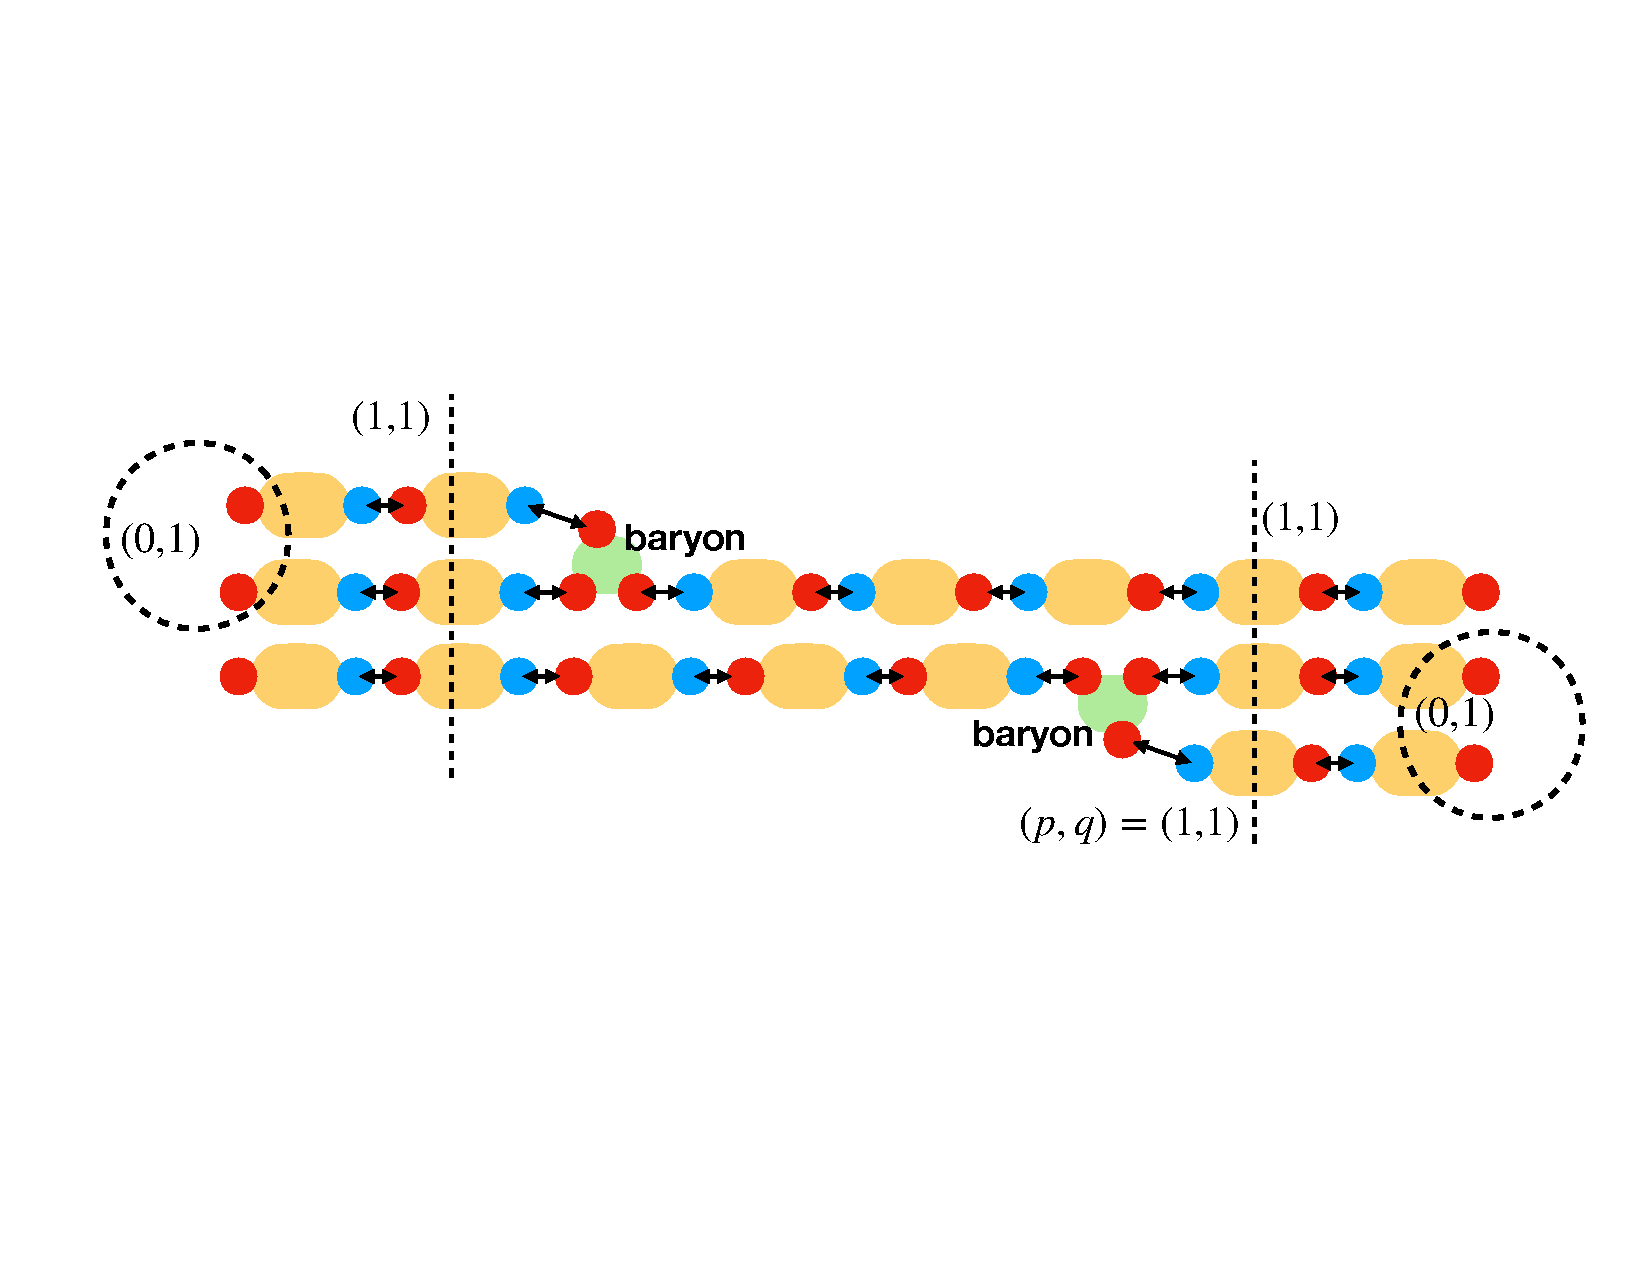
\includegraphics[width=0.6\textwidth]{figs/gluonexchange.pdf}}
\caption{\label{fig:merge}
Upper illustration: The merge of two tubes into one, where the left-hand side tubes begin with two quarks, and the right-hand side ends with one quark. The two quark multiplets couple to a $(0,1)$ multiplet, which then matches with the quark multiplet on the right. The baryon number, is then located at the point where the two tubes merged. This represents a situation where one quark is scattered far, from its original momentum, and the flux tubes must adjust to form local color singlets. The original quark pair must couple to $(p=0,q=1)$ if the overall configuration is to be a color singlet.\\
Lower illustration: This represents the case where two baryons exchange a soft gluon. In that case both of the baryons are transformed into $(p=1,q=1)$ multiplets. Assuming that for each baryon there is a diquark with $(p=0,q=1)$, the overall color singlet is restored by migrating the baryon number to the two places where the strings merge.\\
Darker circles represent quarks, while darker circles represent antiquarks. Ovals represent fluxtubes, and arrows describe quark-antiquark pairs that tunneled from vacuum.
}
\end{figure}


\section{Connecting Baryon Transport to Color Fields}

It is not obvious to see how baryon transport is connected to gluonic fields, $G^{\mu\nu}_a(x)$. Unlike the case for electric fields, gluon fields have a color index, $a$, and because all of nature is in a color singlet, the expectation of the field operators are zero, $\langle G^{\mu\nu}_a(x)\rangle=0$. Therefore, one must describe the fields through operators involving products of operators with color indices, i.e. corrrelators involving two or more operators with color indices. Further, gluons couple to color charge, not to baryon charge. The rather modest goal of this section is to write operators in terms of QCD field operators that represent the baryon polarization or baryon current and the the field-like operators that drive the polarization or current. These operators will be discussed in the context of flux tubes. None of the expressions derived here will be applied to quantitatively predict observables in this study. However, the presentation may help elucidate how fields in QCD can inspire baryon movement and separation.

\subsection{Color-Neutral Correlators}

Here, the color electric/magnetic field operators and the color current operators will be considered, $G^{\mu\nu}_a(x)$, and $j^\mu_a(x)$. Instead of the usual definition of such operators, we add an additional feature that enables the construction of gauge-invariant correlators. For any operator $\mathcal{O}(x)$, an additional attached operator is inferred \cite{Elze:1989un},
\begin{eqnarray}
\mathcal{O}_a(x)&\rightarrow \exp\{i\mathcal{P}\int d\vec{\ell}\cdot\vec{A}\}\mathcal{O}_a(x)\mathcal{P}\exp\{ig\int d\vec{\ell}\cdot\vec{A}\}.
\end{eqnarray}
Here, $\mathcal{P}$ is the path-ordering operator. With this definition, if some correlator $\langle\mathcal{O}_a(x)\mathcal{O}_a(x)\rangle$ is gauge invariant, then $\langle\mathcal{O}_a(x)\mathcal{O}_a(y)\rangle$ is also gauge invariant, though one needs to realize that the new correlator might depend on the actual path chosen. With this definition, one can write expressions that appear similar to those for Maxwell's equations,
\begin{eqnarray}
\partial_\mu j^\mu_a(x)&=&0,\\
\nonumber
\partial_\mu G^{\mu\nu}_a(x)&=&j^\nu_a(x).
\end{eqnarray}
Because all observables must be invariant to rotations in color space, one knows that $\langle\mathcal{O}_a\rangle=0$ and one must consider only colorless correlators. To find quantities which can be treated, at least to some degree, similarly as fields, we consider the following operators defined in terms of operators $j_a^\mu(x)$, where $a$ is a color index. 
\begin{eqnarray}
Q_{a,\Omega}&=&\int d\Omega_\mu j^{\mu}_a(x),\\
\nonumber
\langle Q^{(2)}_{\Omega_1,\Omega_2}\rangle&=&\int d\Omega_{1,\mu}d\Omega_{2,\nu}\langle j^\mu_a(x_1) j^\nu_a(x_2)\rangle,\\
\nonumber
&=&\langle Q_{a,\Omega_1}Q_{a,\Omega_2}\rangle,\\
\nonumber
\langle j^{(2)\nu}_{\Omega_1}(x)\rangle &=&\int d\Omega_{1,\mu} \langle j^\mu_a(x_1) j^\nu_a(x)\rangle\\
\nonumber
&=&\langle Q_{a,\Omega_1}j^\nu_a(x)\rangle.
\end{eqnarray}
Here, the superscripts $(2)$ reference the fact that these correlations are quadratic in the color charge. The volumes $\Omega_1$ and $\Omega_2$ can be any chosen volumes, and might be the same volume. If the volumes cover all space, and if the system is in an overall color singlet, $Q^{(2)}=0$. One can also define correlators using the fields,
\begin{eqnarray}
\langle G^{(2)\mu\nu}_{\Omega}(x)\rangle&=&\int d\Omega\langle Q_{a,\Omega}G^{\mu\nu}_a(x)\rangle.
\end{eqnarray}

As mentioned above, the correlators $\langle\mathcal{O}_a(x)\mathcal{P}_a(x)\rangle$ are gauge-invariant for any operators $\mathcal{O}$ or $\mathcal{P}$ that transform as the color charge, or equivalently as the 8 generators in SU(3). In fact, there are other combinations of operators that transform as color singlets. SU(3) has two Casimir operators, a Casimir being some combination of the group generators that commutes with the eight generators, $\lambda_a$. The first Casimir, often referred to as the quadratic Casimir
\begin{eqnarray}
C^{\rm(quadratic)}&=&\sum_a\lambda_a\lambda_a,
\end{eqnarray}
corresponds to the two-body correlators above. Unlike SU(2), SU(3) has a second Casimir, the cubic Casimir,
\begin{eqnarray}
C^{\rm(cubic)}&=&\sum_{abc}d_{abc}\lambda_a\lambda_b\lambda_c,
\end{eqnarray}
where $d_{abc}$ are the symmetric structure constants.
\begin{eqnarray}
\{\lambda_a,\lambda_b\}&=&\frac{4}{3}\delta_{ab}+d_{abc}\lambda_c.
\end{eqnarray}
It is this second Casimir that will be associated with baryon transport. Once can define a second set of current and charge-like operators, based on the cubic Casimir,
\begin{eqnarray}
\langle j^{(3)\mu}_{\Omega_1,\Omega_2}(x)\rangle &=&d_{abc}\langle Q_{a,\Omega_1}Q_{b,\Omega_1}j^\mu_c(x)\rangle,\\
\nonumber
\langle Q^{(3)}_{\Omega_1,\Omega_2,\Omega_3}\rangle&=&d_{abc}\int d\Omega_{1,\mu}d\Omega_{2,\nu}d\Omega_{3,\eta}\langle j^\mu_a(x_1) j^\nu_a(x_2)j^\eta_c(x_3)\rangle\\
\nonumber
&=&d_{abc}\langle Q_{a,\Omega_1}Q_{b,\Omega_2},Q_{c,\Omega_3}\rangle.
\end{eqnarray}
Again, the three volumes might or might not be the same. One can define the corresponding correlations involving field operators,
\begin{eqnarray}
\langle G^{(3)\mu\nu}_{\Omega_1,\Omega_2}(x)\rangle&=&d_{abc}\langle Q_{a,\Omega_1}Q_{b,\Omega_2}
G^{\mu\nu}_c(x)\rangle.
\end{eqnarray}

For the purposes of this discussion, two vector quantities are defined,
\begin{eqnarray}
E^{(2)}_{\Omega,i}(x)&=&\langle G^{(2)0i}_{\Omega}(x)\rangle,\\
\nonumber
E^{(3)}_{\Omega_1,\Omega_2,i}(x)&=&\langle G^{(3)0i}_{\Omega_1,\Omega_2}(x)\rangle.
\end{eqnarray}
These represent two measures of the color electric field, but are in fact correlators. They have no color index, as their color is defined relative to the color of the matter within the volume $\Omega$. These spatial vectors participate in two versions of Gauss's Law,
\begin{eqnarray}
 \oint d\vec{S}_2\cdot\vec{E}^{(2)}_{\Omega_1}(x_2)&=&Q^{(2)}_{\Omega_1,\Omega_2},\\
 \nonumber
 \oint d\vec{S}_3\cdot\vec{E}^{(3)}_{\Omega_1,\Omega_2}(x_3)&=&Q^{(3)}_{\Omega_1,\Omega_2,\Omega_3}.
\end{eqnarray}
Again, the volumes, $\Omega_1,\Omega_2,\Omega_3$, might or might not be chosen as being the same.

For a flux tube, where the fields are constant across a cross section $\sigma$, one can define a volume $\Omega$ as all tube to the left of some position where we bisect the tube. If the charge with that volume are $Q^{(2)}_{\Omega,\Omega}$, Gauss's law states that the field is 
\begin{eqnarray}
E^{(2)}_{\Omega,\Omega}&=&\frac{1}{\sigma}Q^{(2)}_{\Omega,\Omega}\\
\nonumber
&=&\langle Q_{a,\Omega}E_a\rangle.
\end{eqnarray}
For a single charge $a$, $\langle Q_{a,\Omega}Q_{a,\Omega}\rangle=\langle Q^{(2)}_{\Omega,\Omega}\rangle$. Thus, one can relate the energy density to the fields,
\begin{eqnarray}
 \epsilon&=&\frac{1}{2}\langle E_a^2\rangle\\
 \nonumber
 &=&\frac{1}{2}\frac{(E^{(2)}_{\Omega,\Omega})^2}{Q^{(2)}_{\Omega,\Omega}}.
\end{eqnarray}
The energy per unit length, or string tension is then
\begin{eqnarray}
\frac{E}{L}&=&\frac{\sigma}{2}\frac{(E^{(2)}_{\Omega,\Omega})^2}{Q^{(2)}_{\Omega,\Omega}}\\
\nonumber
&=&\frac{1}{2\sigma}Q^{(2)}_{\Omega,\Omega}.
\end{eqnarray}
Thus, $Q^{(2)}$ is a measure of the energy per unit length of the tube, although if the area changes with the strength of the field, the correspondence is not purely linear.

At the end of this section it will be shown how $Q^{(3)}$ is related to baryon number. The meaning of the two charges are, roughly, that $Q^{(2)}$ describes the energy per unit length of the flux tube and $Q^{(3)}$ represents the propensity of the system to attract baryons vs. antibaryons.

\subsection{Kubo Relations for Conductivity and Polarizability}

Here, we consider a system divided into two volumes, $\Omega$ and a small adjacent volume $\delta\Omega$. We will consider the currents and polarizability in $\delta\Omega$, while using $\Omega$ to define the correlators. The field, $\vec{E}^{(3)}(\vec{r}\in\delta\Omega)$ and the current $\vec{j}^{(3)}(\vec{r}\in\delta\Omega)$ will be defined by the charge distribution in $\Omega$. First, to derive the Kubo relation for the conductivity, we consider the interaction with an color field,
\begin{eqnarray}
H^{\rm(int)}&=&-\int d^3r \rho_a(\vec{r})\vec{r}\cdot\vec{E}_a.
\end{eqnarray}
Following the usual steps for deriving the first-order perturbation correction to the current,
\begin{eqnarray}
\langle\vec{j}^{(3)}_{\Omega\Omega}(\vec{r})\rangle&=&-i\int d^3r'\int_{-\infty}^0 dt~\langle[\vec{j}^{(3)}(\vec{r}),
\int d^3r'~\rho_a(\vec{r}',t)\vec{r}'\cdot\vec{E}_a(\vec{r}',t)]\rangle\\
\nonumber
&=&id_{abc}\int d^3r'\int_{-\infty}^0 dt'~\langle[Q_{a,\Omega}Q_{b,\Omega}\vec{j}_c(\vec{r}),
\int d^3r'~\rho_d(\vec{r}',t')\vec{r}'\cdot\vec{E}_d(\vec{r}',t')]\rangle.
\end{eqnarray}
Here, $\vec{r}$ is inside $\delta\Omega$. Whereas the usual step in deriving Kubo relations is to treat the field as a constant external applied field, here the operator $\vec{E}_{\Omega,\Omega}^{(3)}(\vec{r}')$ is factored out instead. Only the $c=d$ term will contribute in this way.
\begin{eqnarray}
\langle\vec{j}^{(3)}_{\Omega\Omega}(\vec{r})\rangle&=&i\int_{-\infty}^0dt'~\int d^3r'\vec{r}'\cdot
\langle[\vec{j}_a(\vec{r}),\rho_a(\vec{r}',t')]\rangle  \vec{r}'\cdot\vec{E}^{(3)}_{\Omega,\Omega}({\rm in}~\delta\Omega).
\end{eqnarray}
Aside from the color indices, the prefactor to the electric field is the same as for calculating the Kubo relation for a normal electromagnetic field. This yields the result,
\begin{eqnarray}
\langle\vec{j}^{(3)}_{\Omega\Omega}(\vec{r})\rangle&=&\sigma \vec{E}^{(3)}_{\Omega,\Omega}(\vec{r}),\\
\nonumber
\sigma(\vec{r})&=&\frac{1}{2T}\int_{-\infty}^\infty dt'\int d^3r'~\langle\{\vec{j}_{ax}(\vec{r},t=0),\vec{j}_{ax}(\vec{r}',t')\}\rangle.
\end{eqnarray}
Thus, the conductivity, $\sigma$, doesn't include any mention of $\Omega$, and only depends on the local properties. It should be emphasized that Eq. (\ref{eq:jsigmaE}) one describes the contribution to the current due to the charge distribution in $\Omega$. If $\Omega$ is a subvolume, then other regions not only contribute, but their charges might interfere, either constructively or destructively, with those in $\Omega$.

If quarks and gluons are free, one can have currents and fields as presented above. However, if the world is comprised of color singlets, there is no current, but ther can be polarization. As will be discussed in the next subsection, the current $\vec{j}^{(3)}$ is correlated to a baryon current. Similarly, one can define a polarization of the color fields, that is also correlated to the polarization of baryon charge. Here, operators that play the role of polarization, and are also based on the cubic Casimir, are presented. 

The polarization correlator is defined here as
\begin{eqnarray}
\vec{\mathcal{P}}_{\Omega_1,\Omega_2}^{(3)}(\vec{r})=\vec{r}d_{abc}\langle Q_{a,\Omega_1}Q_{b,\Omega_2}\rho_c(\vec{r})\rangle.
\end{eqnarray}
Using the same interaction as was used for the calculation of the conductivity above, one can calculate the thermal expectation of the polarization. Setting $\Omega_1=\Omega_2=\Omega$, and factoring out $E^{(3)}$ as was done earlier, one finds
\begin{eqnarray}
\vec{\mathcal{P}}_{\Omega,\Omega}^{(3)}(\vec{r})&=&\kappa \vec{E}^{(3)}_{\Omega,\Omega}(\vec{r}),\\
\nonumber
\kappa(\vec{r})&=&\frac{1}{3T}\int d^3r'\langle \rho_a(\vec{r})[\vec{r}\cdot\vec{r}']\rho_a(\vec{r}')\rangle.
\end{eqnarray}
As was the case for the conductivity, this expression for the polarizability does not depend on the the volume $\Omega$. If the charges appear in uncorrelated $\pm$ pairs, the polarizability becomes $g^2\langle(x_+-x_-)^2\rangle\rho_d$, where $\rho_d$ is the density of dipoles and $x_+-x_-$ is the distance between the two charges, $\pm g$. 


\subsection{Relation to Baryon Transport}

As was promised previoisl, the goal of this subsection is to demonstrate how baryon transport is related to the field $\vec{E}^{(3)}$, which was in turn related to the cubic Casimir. The quadratic and cubic Casimirs can be expressed in terms of the color multiplet labels $p$ and $q$ through
\begin{eqnarray}
C^{\rm quadratic}&=&(p^2+q^2+3p+3q+pq)/3.0,\\
C^{\rm cubic}&=&(p-q)(2p+q+3)(2q+3q+3).
\end{eqnarray}
The multiplet labels $p$ and $q$ and the charge labels $Q^{(2)}$ and $Q^{(3)}$ represent alternative means to identify the multiplet. The labels $p$ and $q$ can be uniquely expressed in terms of the charges by solving a cubic equation. Defining
\begin{eqnarray}
c&\equiv&-9Q^{(2)}-9,\\
\nonumber
d&\equiv&18Q^{(3)},\\
\nonumber
\alpha&=&-2\pi /3+\frac{1}{3}\cos^{-1}[(3d/2c)\sqrt(-3/c)],\\
\nonumber
y&=&2\sqrt{-c/3}\cos[\alpha],\\
\nonumber
x&=&-2+\sqrt{4+Q^{(2)}-y^2/3},\\
\nonumber
p&=&(x+y)/2,\\
\nonumber
q&=&(x-y)/2.
\end{eqnarray}
The other two solutions to the cubic equation result in either $p$ or $q$ being negative. The solutions are unique in that no two combinations of  $Q^{(2)}$ and $Q^{(3)}$ result in the same $p$ and $q$.

Given that a quark has $p=1,q=0$ and an antiquark has $p=0,q=1$, it is natural to expect that a multiplet with $p>q$ will more likely dissolve into quarks, and that a multiplet with $q>p$ would more likely result in antiquarks.



\begin{acknowledgments}
This work was supported by the Department of Energy Office of Science through grant number DE-FG02-03ER41259.
\end{acknowledgments}

\bibliography{btransport}

\end{document}
